\documentclass[notitlepage]{article}

\usepackage{graphicx}
\usepackage{caption}
\usepackage{rotating}
\usepackage{float}
\usepackage[margin=0.8in]{geometry}
\usepackage[section]{placeins}
\usepackage[hidelinks]{hyperref}
\usepackage{bytefield}
\usepackage{sectsty}
\sectionfont{\clearpage}
\usepackage{csquotes}
\MakeOuterQuote{"}

\setlength{\parskip}{0.3em}
\usepackage{xcolor}
\usepackage{listings}
\lstset{
	language=Verilog,
	frame=single,
	basicstyle=\small,
	keywordstyle=\color{blue}\small,
	stringstyle=\color{Maroon}\small,
	commentstyle=\color{OliveGreen}\small,
	breaklines=true,
	postbreak=\raisebox{0ex}[0ex][0ex]{\ensuremath{\color{red}\hookrightarrow\space}}
}

\title{RISCBoy Documentation}
\author{Luke Wren}
\makeatletter
\newcommand*{\toccontents}{\@starttoc{toc}}
\makeatother

\begin{document}

\pagenumbering{gobble}
\maketitle
\toccontents
\listoffigures
\newpage
\pagenumbering{arabic}

\section{Introduction}

RISCBoy is an open source portable games console, designed from scratch:

\begin{itemize}
\item An open source CPU, graphics and bus architecture
\item Based on the RISC-V open source instruction set
\item FPGA synthesis, place and route with icestorm open source FPGA toolchain
\item An open source PCB layout
\item PCB designed with KiCAD open source PCB software
\item It's open source
\end{itemize}

\begin{displayquote}
{\it If you say open source one more time I'm gonna nut instantly} - Oscar Wilde
\end{displayquote}

\subsection{Digital Design}

\begin{figure}[!htb]
\caption{System-level block diagram}
\label{diagram:system_arch}
\centering
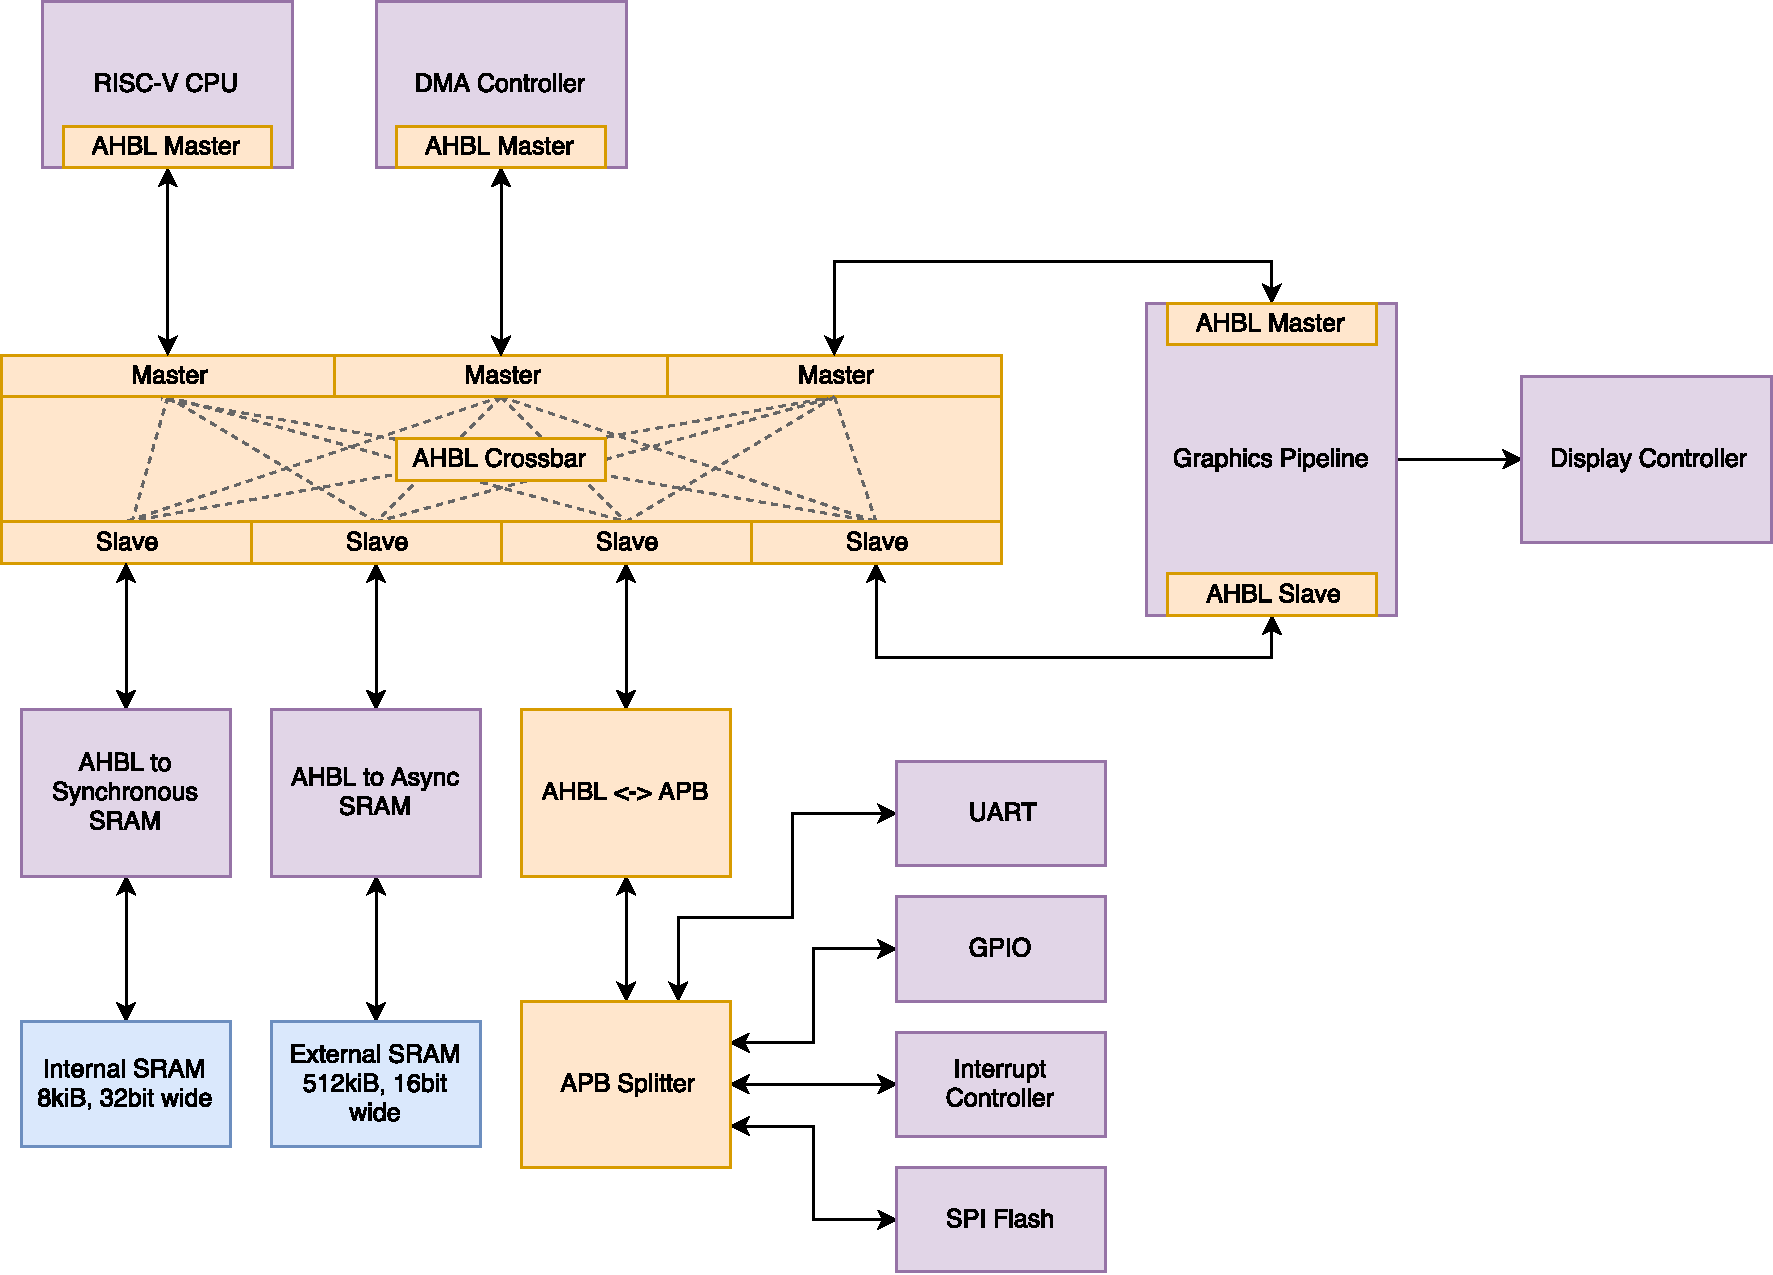
\includegraphics[width=0.7\textwidth]{diagrams/system_arch.pdf}
\end{figure}

The heart of the design is a Lattice iCE40-HX8k FPGA, containing 7680 LUT4s and flipflops. The logic was designed in synthesisable Verilog, with no dependencies on FPGA vendor IP; the contents of this GitHub repository could be taped out onto a chip. This includes:

\begin{itemize}
\item RV32IC-compatible 32-bit CPU design
	\begin{itemize}
	\item RISC-V instruction set
	\item 32I: base integer ISA profile
	\item C: compressed instruction extension, for higher code density
	\item Vectored interrupts (save/restore of PC, RA only)
	\item 5-stage pipeline, similar to textbook RISC
	\item Single AHB-Lite master port
	\end{itemize}
\item Graphics pipeline
	\begin{itemize}
	\item Don't expect much, it's about as powerful as a Gameboy Advance
	\item Includes some MODE7-like functionality which allows drawing perspective-mapped textured planes, by providing per-scanline affine texture transformation. Think MarioKart
	\end{itemize}
\item AMBA 3 AHB-Lite compatible multi-master busfabric
\item Peripherals:
	\begin{itemize}
	\item DMA master
	\item External asynchronous SRAM controller (GS74116 or similar)
	\item Display controller (ILI9341)
	\item GPIO (bitbanging, peripheral muxing)
	\item SD card controller
	\item UART
	\item PWM
	\item Basic audio: voices + samples, noise-shaped PWM output
	\end{itemize}
\end{itemize}

This document attempts to describe some of these, but if you need nitty-gritty detail, the best documentation is the files ending with {\tt .v}.

That a free synthesis tool can cram this into one of the cheapest FPGAs on the market is tremendous. I hope for a situation like software compilers, where free tools such as GCC and LLVM are industry standards.

\subsection{PCB}


\begin{figure}[!htb]
\centering
\caption{PCB stackup (left), and BGA-to-via critical clearances and dimensions (right)}
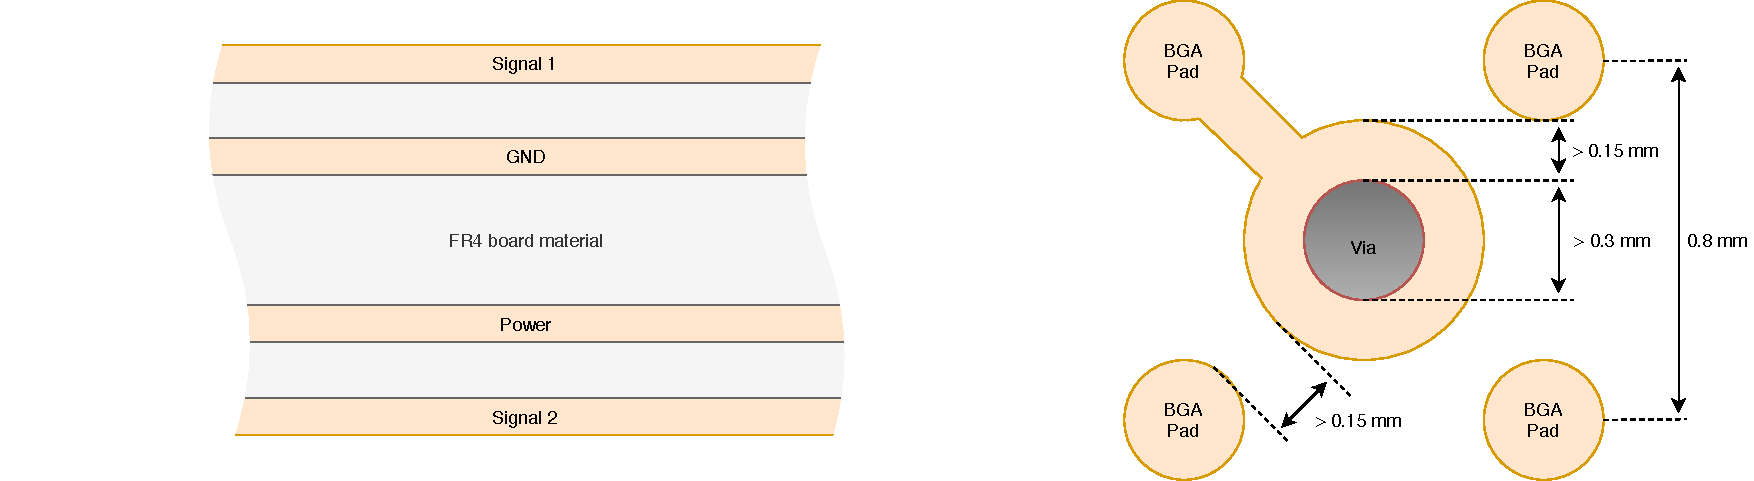
\includegraphics[width=0.8\textwidth]{diagrams/stackup_and_bga.pdf}
\label{diagram:stackup_and_bga}
\end{figure}

The board has a 4-layer stackup, illustrated in figure \ref{diagram:stackup_and_bga}. It targets low-cost PCB prototyping services such as iTead, and makes compromises to achieve this, chiefly escape routing from the FPGA ($11 \times 11$ 0.8 mm BGA). To meet iTead's copper-clearance, minimum via drill, and minimum annular ring specifications, the BGA pads must be sized down to 0.23 mm. Reflow this component by hand, with a hot air gun and plenty of flux; your toaster oven isn't going to cut it.

Schematic and layout files are in the {\tt board/} subdirectory of the git repository.

\subsection{Licensing}

The Verilog source to this project has no dependencies, and is distributed under the DWTFPL version 3. This is a {\it very} permissive open-source licence, and its text is included in full at the top of the source files. This license is very similar to the original DWTFPL, which more readers may be familiar with, but has an added indemnification clause.

This license is also known by its more formal name, as the "Do What The Fuck You Want To And Don't Blame Us Public License".

\section{CPU Architecture}

Hazard5 is a 32-bit processor based on the RISC-V instruction set architecture. It accesses the system through a single AMBA 3 AHB-Lite master port. Those familiar with the textbook 5-stage RISC pipeline will find Hazard5 mostly straightforward, but hopefully will still find some interesting tricks. We will use the following symbols to refer to the 5 stages:

\begin{itemize}
\item {\tt F}: fetch
\item {\tt D}: decode
\item {\tt X}: execute
\item {\tt M}: memory access (load/store)
\item {\tt W}: register writeback, fetch address generation
\end{itemize}


Hazard5 supports the RV32IC instruction set, whose encoding is variable-width. The C extension typically reduces instruction bandwidth by \textasciitilde 25\%, which helps to maintain performance when sharing bus access between fetch and load/store.

Branches are speculated, but there is currently no dynamic branch predictor. Instead, we use the static prediction scheme described in the RV ISA manual (based on sign of branch offset).

% \newpage

% \begin{center}
% 	\begin{sideways}
% 		\begin{minipage}{\textheight}
% 			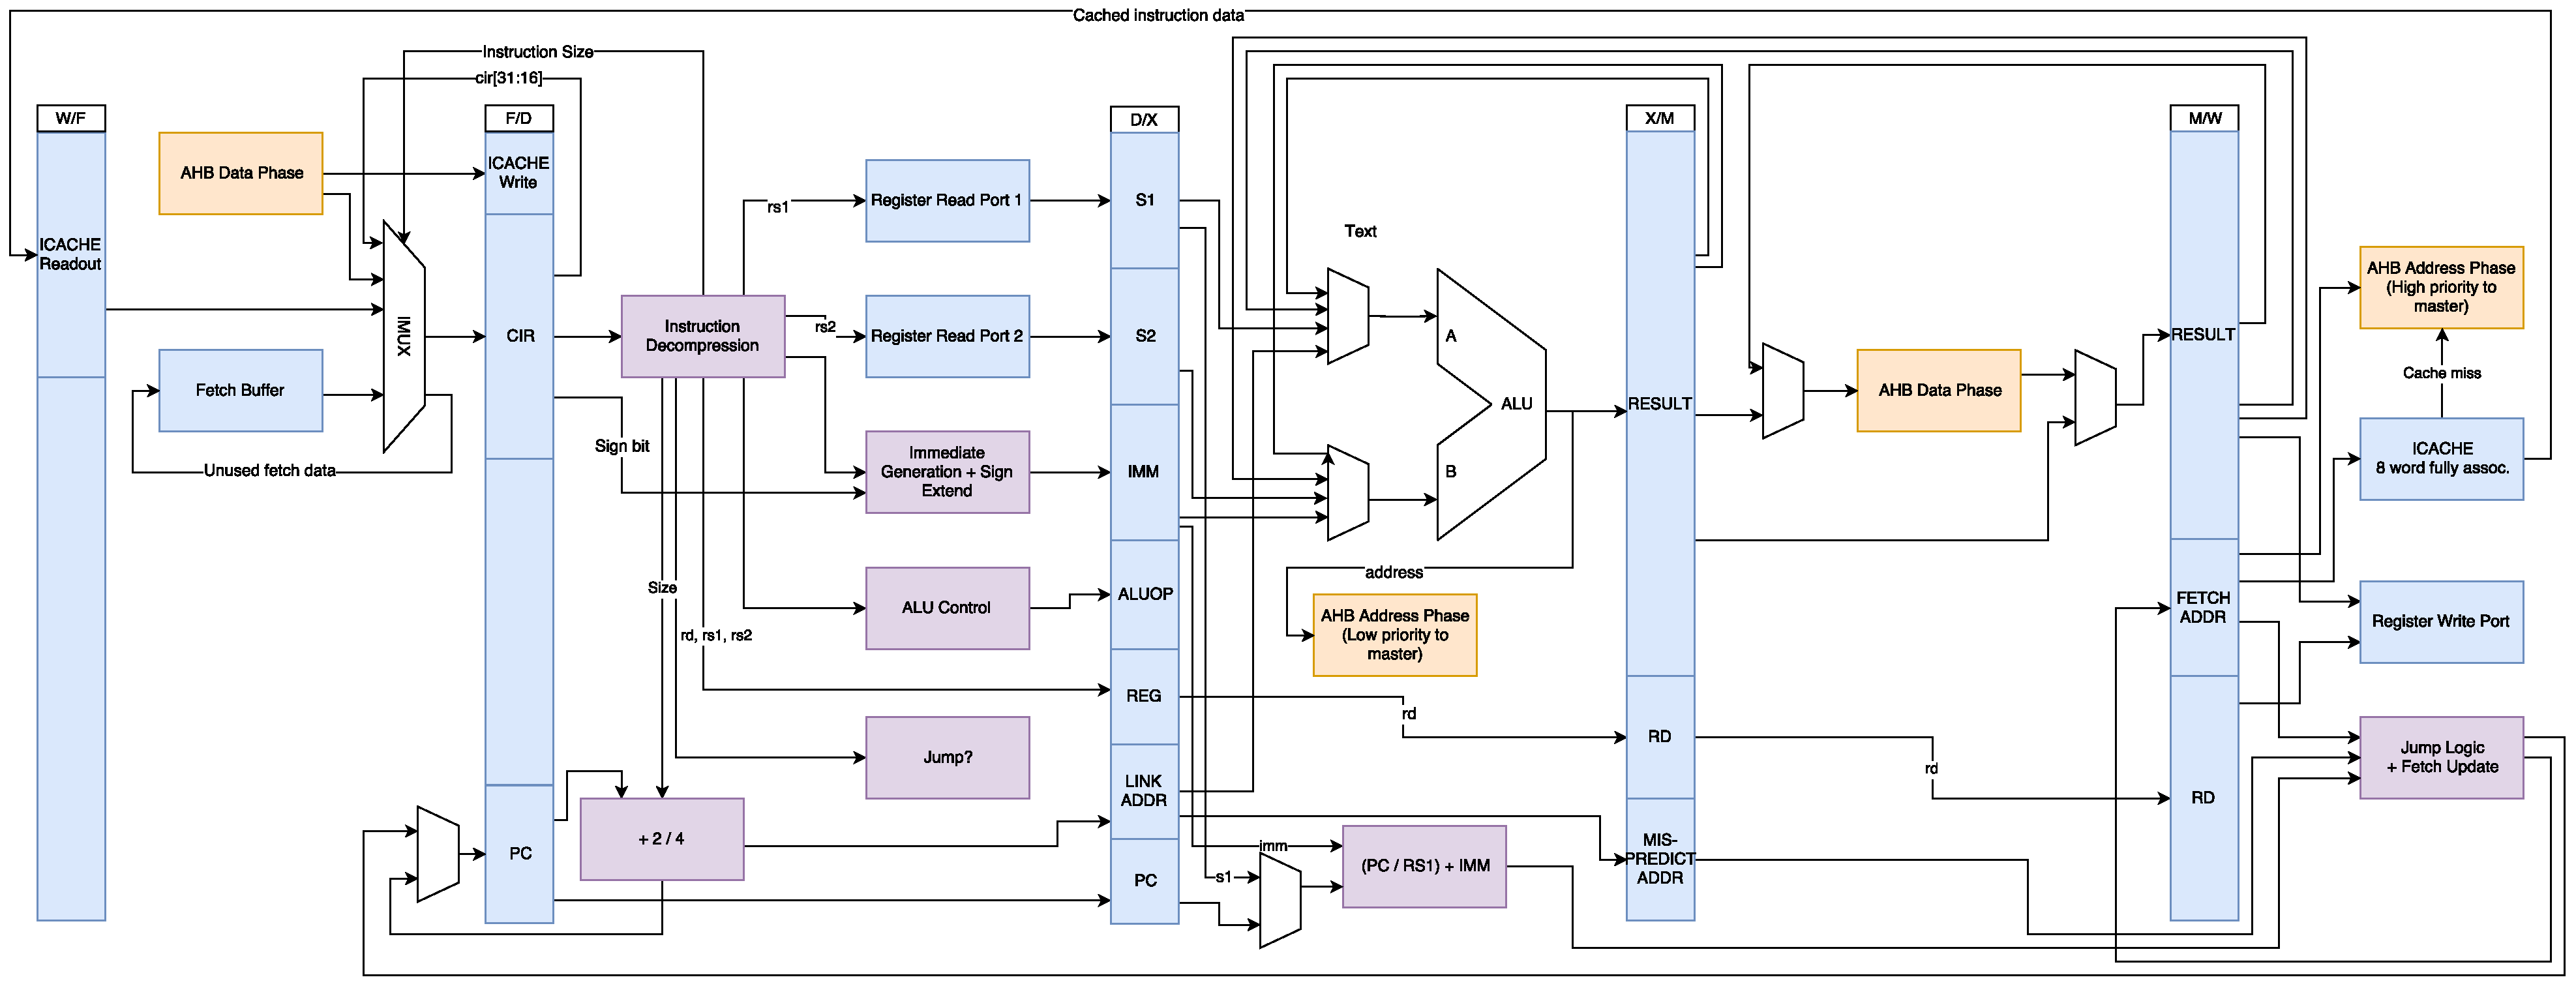
\includegraphics[width=\textheight]{diagrams/cpu_full.pdf}
% 			\captionof{figure}{Hazard5 architectural block diagram}
% 			\label{diagram:cpu_pipeline}
% 		\end{minipage}
% 	\end{sideways}
% \end{center}

% \newpage

\subsection{Frontend}
\label{section:frontend}

\begin{figure}[!htb]
\centering
\caption{Hazard5 processor frontend, block diagram}
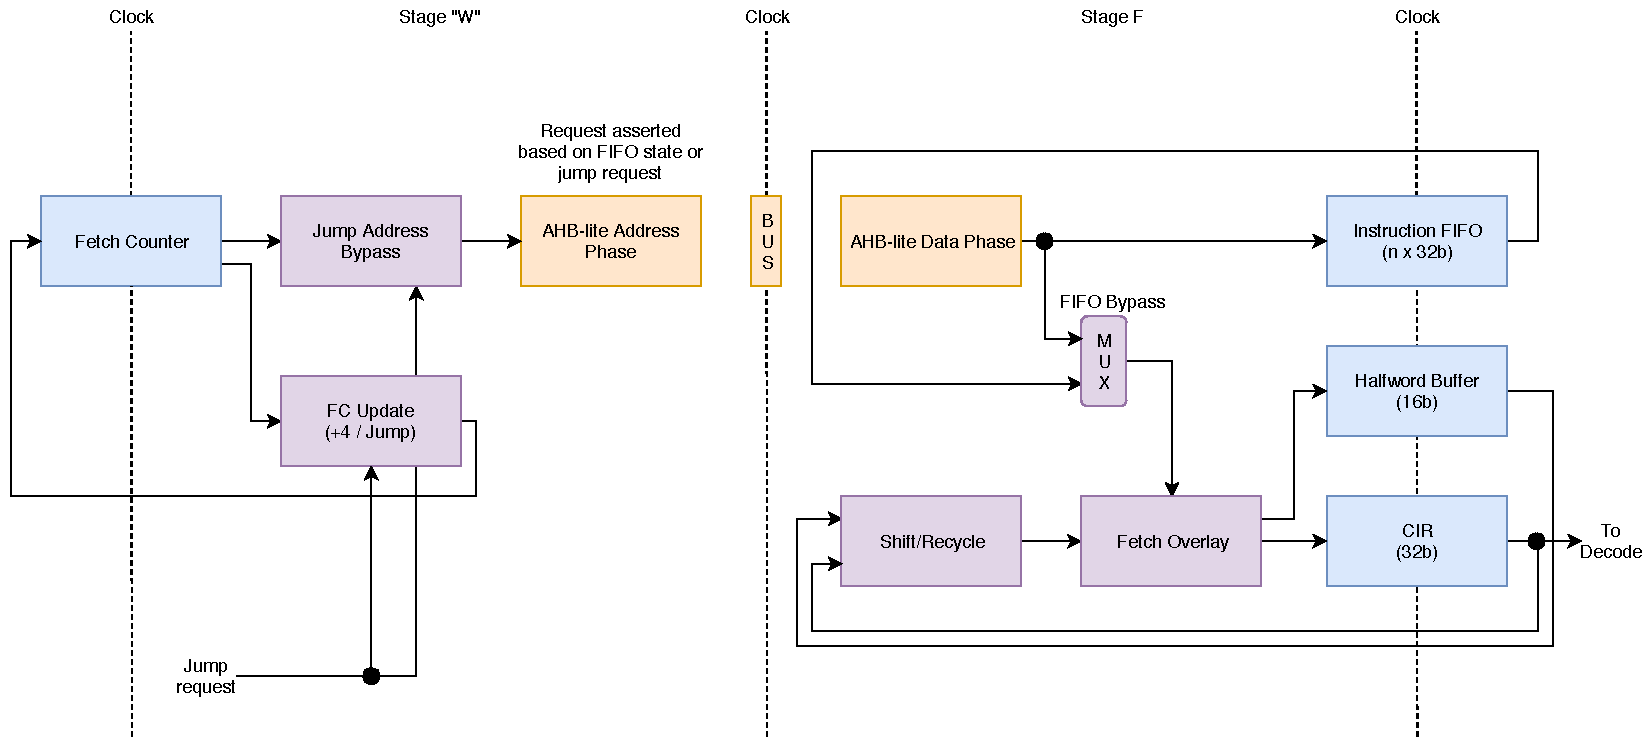
\includegraphics[width=0.9\textwidth]{diagrams/cpu_frontend.pdf}
\label{diagram:frontend}
\end{figure}

The frontend (figure \ref{diagram:frontend}) consists of stage {\tt F} and an additional stage which performs the AHB address phase, and can be considered part of {\tt W}. Its purpose is to feed {\tt D} with instructions, whilst meeting the following constraints:

\begin{itemize}
	\item No combinatorial path from AHB-Lite data phase to address phase (e.g. {\tt hready} $\to$ {\tt htrans})
	\item AHB-Lite compliant: no unaligned transfers, no deassertion or change of active requests
	\item Provide up to 32 bits of instruction data per clock in steady state, even if instructions are unaligned
	\item 0-cycle jump/flush to AHB address phase assertion (with minimal logic on this path)
	\item No performance penalty for unaligned jump to 16-bit instruction
	\item Attempt to maintain performance when competing with the load/store unit and AHB-Lite busmaster peers
\end{itemize}

The main source of complexity is that a RISC-V *C instruction stream is not naturally-aligned, i.e. instruction address modulo instruction size is not always zero. We spend gates here to optimise the common case of sequential execution, and to lessen the effects of fetch starvation due to load-store activity.

To meet these constraints, the frontend performs almost exclusively word accesses, which must be aligned. The only exception is a jump (or similar, e.g. mispredict recovery) to a non-word-aligned address. In this case, a halfword fetch from the target address is performed.

\subsubsection{Prefetch Queue}

The frontend queues up fresh instruction data which is waiting to be decoded. The pipelined nature of AHB-Lite means that the bus transfers run ahead of {\tt D} by at least two clocks, and the prefetch queue is able to buffer these in-flight transfers if {\tt D} stalls against a later pipe stage. The queue also decouples {\tt D}'s stall logic (which is a function of {\tt hready}) from the address phase request, and finally, the queue helps keep {\tt D} supplied with instructions while the busmaster is busy with load/stores from {\tt X}.

There are three parts to the queue:

\begin{itemize}
	\item A 32-bit FIFO. The depth is configurable, and can be as little as 1 word.
	\item A halfword buffer which may store the higher-addressed half of a recently-popped FIFO word
	\item The upper half of the current instruction register ({\tt CIR}), if the previous instruction was 16-bit
\end{itemize}

These three sources should service the majority of instruction fetches, and fresh bus data is written only to the FIFO. However, following jumps, flushes, or fetch starvation (either due to load/store activity or bus wait states), bus data can be forwarded directly to {\tt CIR}.

\subsubsection{Program Counter}

Hazard5 does {\it not} use the program counter ({\tt PC}) for code fetching, during sequential execution. {\tt PC} is used exclusively for the link value in {\tt JAL(R)}, mispredict recovery, and PC-relative addressing; it is physically located in {\tt D}.

The frontend fetches instruction data from consecutive word-aligned addresses, paced by backpressure from the instruction FIFO; {\tt PC} is not involved. However, as a special case, it {\it does} need the full jump target address (which becomes the new {\tt PC}), as unaligned jumps require special attention.

\subsubsection{Arbitration of Fetch and Load/Store}
\label{section:fetch_ls_arb}

The single AHB master port asserts transactions from two sources: the frontend, whose address phase is in {\tt W}, and the load/store unit, whose address phase is in {\tt X}. Frontend requests may be linear or non-linear (e.g jumps). The rules are:

\begin{enumerate}
	\item If a jump or mispredict recovery is asserted by {\tt M}, this wins.
	\begin{itemize}
		\item Any requests from earlier stages are logically later in program order.
		\item If {\tt M} wants to jump then these instructions are being executed in error, so should certainly not be permitted to access the bus.
	\end{itemize}
	\item Else if a load/store is asserted by {\tt X}, this wins.
	\begin{itemize}
		\item Stalling instruction fetch {\it may} be covered by the prefetch queue, in which case we've lost nothing
		\item Stalling a load/store will always increase execution time
		\item If instead {\tt X} stalled, and instruction fetch ran ahead, what would we do with the fetched instructions?
	\end{itemize}
	\item Otherwise, perform any other access requested by the frontend.
	\begin{itemize}
		\item Always Be Fetching
	\end{itemize}
\end{enumerate}

The fetch and load/store interfaces are well-decoupled; it would be simple to remove the arbiter and create a 2-master processor configuration. (TODO: add a wrapper that does this!)

\subsubsection{Jumps and Branches}

Due to the pipelined nature of AHB, we are unable to jump or to take branches in fewer than 2 cycles (without adding sophisticated prediction):

\begin{itemize}
\item Cycle 0: AHB data phase for fetch of jump/branch. Next instruction is in address phase concurrently.
\item Cycle 1: Jump/branch instruction is now available to {\tt D}
	\begin{itemize}
		\item (Quickly) use to control the new address phase
		\item The immediately following instruction is already in data phase
	\end{itemize}
\item Cycle 2: Data phase for jump target instruction
\item Cycle 3: Jump target is presented to {\tt D} and decoded.
\end{itemize}


We knew the jump target on cycle 1, but did not begin decoding the targeted instruction until cycle 3. We also made one wasted code fetch. This is suboptimal, but fetching the jump target {\it before} decoding the jump is tricky, and there are lower-hanging fruit in terms of performance per LUT.

Jumps physically occur in {\tt W}, directly in front of the fetch address generator. There are two reasons to jump:

\begin{itemize}
	\item Inspecting the {\tt CIR} in {\tt F/D} pipe register ({\tt JAL}, speculated taken branches)
	\item Inspecting {\tt X/M} pipe register ({\tt JALR}, branch mispredict recovery)
\end{itemize}

{\tt JALR} (indirect jump) is taken later because it uses the register file and the ALU to compute its target.

If both of these sources attempt to jump in the same cycle, {\tt X/M} takes priority, since it is executing an older instruction. In both cases, the part of the pipeline in the hazard shadow is invalidated; i.e., {\tt W} $\to$ {\tt F}, or {\tt W} $\to$ {\tt X}. Invalidation is performed by clobbering the pipeline control signals in such a way that these instructions will have no side effects.

The branch prediction scheme is static: take backward branches, and do not take forward branches. The cycle costs are as follows:

\begin{center}
\begin{tabular}{l c}
\hline
Jump Type & Cycles (Execution + Penalty) \\
\hline
Direct jump & 2 \\
Predicted, non-taken branch & 1 \\
Predicted, taken branch (same as jump) & 2 \\
Indirect jump & 4 \\
Branch mispredict & 4 \\
\hline
\end{tabular}
\end{center}

Upon jumping, we need some mechanism to invalidate parts of the pipeline: this is described in section \ref{section:stalling_flushing}.

\subsubsection{CIR Locking}

There is a landmine in the following tableau:

\begin{itemize}
	\item {\tt M} contains a load (in data phase), and the bus is stalled
	\item {\tt X} contains an instruction dependent on the load result; say an {\tt AND}
	\item {\tt D} contains a branch which is mispredicted taken
\end{itemize}

For example, say we are polling a status bit in an IO register, looping until some bit is high. The instruction in {\tt X} must stall for at least two cycles due to the bus stall and load-use hazard. Due to a frontend design constraint from \ref{section:frontend} -- "No combinatorial path from AHB-Lite data phase to address phase (e.g. {\tt hready} $\to$ {\tt htrans})" -- we must not use {\tt X}'s stall signal to gate the jump request, as this would create such a path. However, {\it not} gating the jump request is fatal, as new fetches will clobber {\tt CIR} before the branch instruction can proceed into {\tt X}, so the mispredict will never recover. {\tt JAL} has the same problem: it will jump, but not produce a link address.

Hazard5 resolves this with {\tt CIR} locking. {\tt D} signals to {\tt F} that {\tt CIR} and its validity count must not change on the next clock edge, and uses this same signal to inhibit repeated assertion of its own jump request. In the fetch path, this is achieved by steering the controls on the existing shift/overlay logic in the frontend, and requires no additional muxing.

Whilst the {\tt CIR} is locked, the frontend is still free to act on the jump request, and fetch ahead along the new code path (more useful for {\tt JAL}); this data is buffered in the FIFO. Once the roadblock ahead of {\tt D} clears, the branch instruction proceeds down the pipeline, and the lock is released simultaneously.

Note also that a bus stall does not cause the frontend to block jump requests, as this too would create a combinatorial path, since requests are forwarded straight to the bus (due to another constraint from \ref{section:frontend}). The frontend's response to bus stall on jump request is simply to not increment the target before storing to {\tt FC}, so that the target address continues to be asserted on subsequent cycles. Registered feedback blocks {\it subsequent} jump requests until the first request completes its address phase.

\subsubsection{Instruction Barrier (FENCE.I)}

If the program stores to instruction addresses about to be executed from, which potentially exist in the prefetch queue, a stale instruction will be executed. {\tt FENCE.I} cannot be decoded as a nop, and requires special handling.

Hazard5 decodes {\tt FENCE.I} as "jump to {\tt PC} + 4". The jump invalidates the prefetch queue, and the following instruction will be re-fetched from memory.

Timing analysis shows that calculating a jump target, between {\tt CIR} and the address bus, is generally on the critical path. To avoid more logic on this path, {\tt FENCE.I} is instead implemented by spoofing a branch-taken mispredict, which has the same effect. This adds two cycles to the execution time, but performance of this instruction is decidedly noncritical.

\subsection{Operand Bypass}

Hazard5 possesses an operand bypass (forwarding) network. Register writes by one instruction must always be visible to later instructions, even before the first instruction reaches register writeback. This is shown as multiplexers on the ALU inputs in figure \ref{diagram:cpu_pipeline}.

This reduces (and often eliminates) the penalty of read-after-write data hazards in the pipeline, and allows us to approach one-clock-per-instruction (CPI) execution rates. Without bypass, only one instruction could exist present in $\left\{ {\tt D}, {\tt X}, {\tt M}, {\tt W} \right\}$ at a time, giving a CPI of 4.

The following bypasses are available: (notation: pipe register $\to$ pipestage logic)

\begin{itemize}
	\item {\tt X/M} $\to$ {\tt X}
	\item {\tt M/W} $\to$ {\tt X}
	\item {\tt M/W} $\to$ {\tt M}
	\item {\tt W/X} $\to$ {\tt X}
\end{itemize}

The last is in lieu of a write-to-read bypass in the register file, to avoid difficulties with block-RAM inference on iCE40.

To control the bypassing, some of the register specifiers from {\tt CIR} are passed down the pipeline alongside the data. {\tt rs1, rs2, rd} (operand sources and destination) are passed down as far as {\tt X}. {\tt rs2, rd} make it to {\tt M}, and only {\tt rd} makes it to {\tt W}.

The upshot is:

\begin{itemize}
	\item Back-to-back ALU operations execute at 1 CPI
	\item Loads insert 1 stall cycle if immediately required by the ALU. 1 CPI otherwise.
	\item Stores execute at 1 CPI (bus stall notwithstanding)
	\item In a load + store pair, the load takes only one cycle, since the {\tt M} stage has self-forwarding
\end{itemize}

Various interesting strategies can alleviate load-use penalty in in-order pipelines, such as adding a second, "late" ALU in the {\tt M} stage. In our case we judge this to not be worth the LUTs.

\subsection{Pipeline Stalling and Flushing}
\label{section:stalling_flushing}

Our terminology: stalling means a pipeline stage does not advance its state until some blocking condition has cleared. The instruction residing in this stage will not progress to the next stage, and the previous stage will not write {\it its} instruction into this stage. Flushing is when in-flight instructions in some stages are replaced with NOPs, and their results are discarded.

The frontend is decoupled from other stages' stall logic via the prefetch queue. This is important: {\tt hready} is an input to that stall logic, and the the frontend's address-phase request must not be a function of {\tt hready}.

The frontend may not be able to immediately accept a jump request, which may cause other pipe stages to stall if it is low. One cause is the frontend holding an existing address-phase request stable until the cycle {\it after} {\tt hready}, which is required for AHB-Lite compliance.

For the backend, the stall logic is more intricate, as signals such as {\tt hready} are used in-cycle to determine whether an instruction progresses to the next pipeline stage:

\begin{itemize}
	\item {\tt D}:
	\begin{itemize}
		\item {\tt CIR} does not contain a valid instruction (either no data, or half of a 32-bit instruction)
		\item {\tt D} asserts jump, but frontend rejects the jump request
		\item {\tt X} is stalled
	\end{itemize}
	\item {\tt X}:
	\begin{itemize}
		\item {\tt hready} low and {\tt X} address-phase request asserted
		\item RAW hazard on {\tt M} (load-use)
		\item {\tt M} is stalled
	\end{itemize}
	\item {\tt M}:
	\begin{itemize}
		\item {\tt hready} low and data-phase active
		\item {\tt M} asserts jump, but frontend rejects the jump request
	\end{itemize}
	\item {\tt W}: does not stall
\end{itemize}

If a given stage is stalled, but the following stage is not, it must insert a bubble. Bubbles are created by zeroing out control fields, such as {\tt rd}, so that the instruction cannot affect system or processor state.

There are two cases where we must flush:

\begin{itemize}
	\item Branch/jump taken from {\tt D}; frontend invalidates prefetched data
	\item Jump/mispredict taken from {\tt M}; must flush frontend, {\tt D}, {\tt X}
\end{itemize}

And the flushing mechanisms for each stage are as follows:
\begin{itemize}
	\item {\tt D}: destination register {\tt rd} cleared, which makes result invisible to register file and operand bypass. {\tt memop}, {\tt branchcond} pipe flags are cleared.
	\item {\tt X}: same as {\tt D} (except for {\tt branchcond}, which does not pass on to {\tt M} anyway.
\end{itemize}

Flushing and bubble insertion are very similar in mechanism.

\subsection{Unaligned Memory Accesses}

Alignment is the constraint that the address of a memory access be equal to zero, modulo some size. Where no size is specified, we refer to {\it natural} alignment, i.e. modulo the size of this particular memory operation. RISC-V requires that memory is byte-addressable.

The frontend goes to some length (section \ref{section:frontend}) to maintain high throughput. RV-C instruction streams are {\it always} unaligned, and {\it every} instruction must be fetched before it is executed, so Amdahl says it's worth it.

As load/stores are less than 100\% of all instructions, and generally much fewer than 100\% of these are unaligned, Hazard5 does not have hardware support for unaligned load/stores. These are trapped (TODO) and handled in software if and when they occur.

\subsection{Interrupts and Exceptions}

This section is very much still TBD. (TODO)

Hazard5 will have non-nested priority vectored interrupts, with no register saving, apart from {\tt ra} ({\tt x2}; link/return address register) and the {\tt PC}. Interrupts and exceptions will be implemented with the early jump hardware, so behave as a {\tt D}-sourced jump.

Interrupts/exceptions are implemented as a jump into the vector table. The table is a block of aligned 32-bit instructions, which will most likely be JAL, meaning ISRs must be within $\pm$1 MiB of the vector table. As well as jumping into the table, the interrupt hardware stashes the {\tt PC} and {\tt ra} into shadow registers; the second requires a register file read, and the pipeline slot of the (victim) instruction in {\tt D} is used to perform this read. {\tt PC} is immediately clobbered by the jump into the table, and {\tt ra} is clobbered with the magic value 0xffffffff, which is otherwise an invalid return address as its LSB is set.

Upon encountering a {\tt jalr} to 0xffffffff (most likely a {\tt ret}), the saved {\tt PC} and {\tt ra} are saved.

Consequently, ISRs may not generate exceptions, such as unaligned accesses. TODO: should have some kind of non-returning hardfault exception to deal with things like this.

\subsection{Plugin Interface}

Plugins are pieces of hardware attached to the Hazard5 pipeline to extend its functionality, and instruction set. For example, the M extension (multiply and divide) is implemented using a plugin.

Plugins interact with three pipe stages:

\begin{itemize}
	\item {\tt D}
	\begin{itemize}
		\item Plugins see the current instruction, so that they can decode it
		\item Plugins notify {\tt D} that an instruction it does not recognise is, in fact, valid
	\end{itemize}
	\item {\tt X}
	\begin{itemize}
		\item Plugins can see the {\tt rs1} and {\tt rs2} operand bypasses
		\item Additional control signals provide functionality such as killing an in-progress operation so that e.g. an interrupt can run
	\end{itemize}
	\item {\tt M}
	\begin{itemize}
		\item All plugins retire their results into {\tt M}.
		\item This adds a 1-cycle RAW stall if the immediately-following instruction is dependent, but on current iCE40 implementations, {\tt X} is already near-critical-path and very mux heavy.
		\item Plugins can stall {\tt M} if they need more cycles to produce a result.
	\end{itemize}
\end{itemize}

There is no hard limit to the number of plugins that can be added, but the additional muxing and fanout is not free, which constrains practical implementations.

\subsubsection{M-small Plugin}

The M-small plugin implements the RISC-V M standard extension (multiply and divide). To save area, the plugin employs a combined multiply/divide unit which performs the required calculations at 1 bit per clock.

\subsubsection{M-fast Plugin}

The Mfast plugin also implements the M extension, but uses a fast Wallace tree to perform multiplication, allowing a throughput of 1 32-bit multiply per clock.

Other details TBD

\section{Bus Fabric and Memory Subsystem}

Bus fabric is digital plumbing. A master, such as a processor, requests a read or write on some address; the bus fabric routes the request to the correct slave device, and routes the response back. RISCBoy implements two bus fabric standards:

\begin{itemize}
\item AMBA 3 AHB-Lite connects masters to high-performance devices such as SRAM controllers
\item AMBA 3 APB connects to simple devices such as a UART
\end{itemize}

Figure \ref{diagram:crossbar_structure} shows the structure of the AHB-Lite crossbar ({\tt ahbl\_crossbar.v}). The crossbar is shown in context in figure \ref{diagram:system_arch}. An independent AHB-Lite datapath connects each of $m$ masters to each of $n$ slaves. One master can address one slave at a time, and one slave can be in data-phase with one master at a time; subject to these constraints, up to $\min(m,n)$ independent transfers can take place in a single machine clock cycle.

Some claim AHB-Lite does not "support" multi-master arbitration. Their problem is a lack of enthusiasm: motorbikes do not "support" wheelies by design, but are excellent at it.

\begin{figure}[!htb]
\centering
\caption{AHB-Lite crossbar, module-level block diagram} 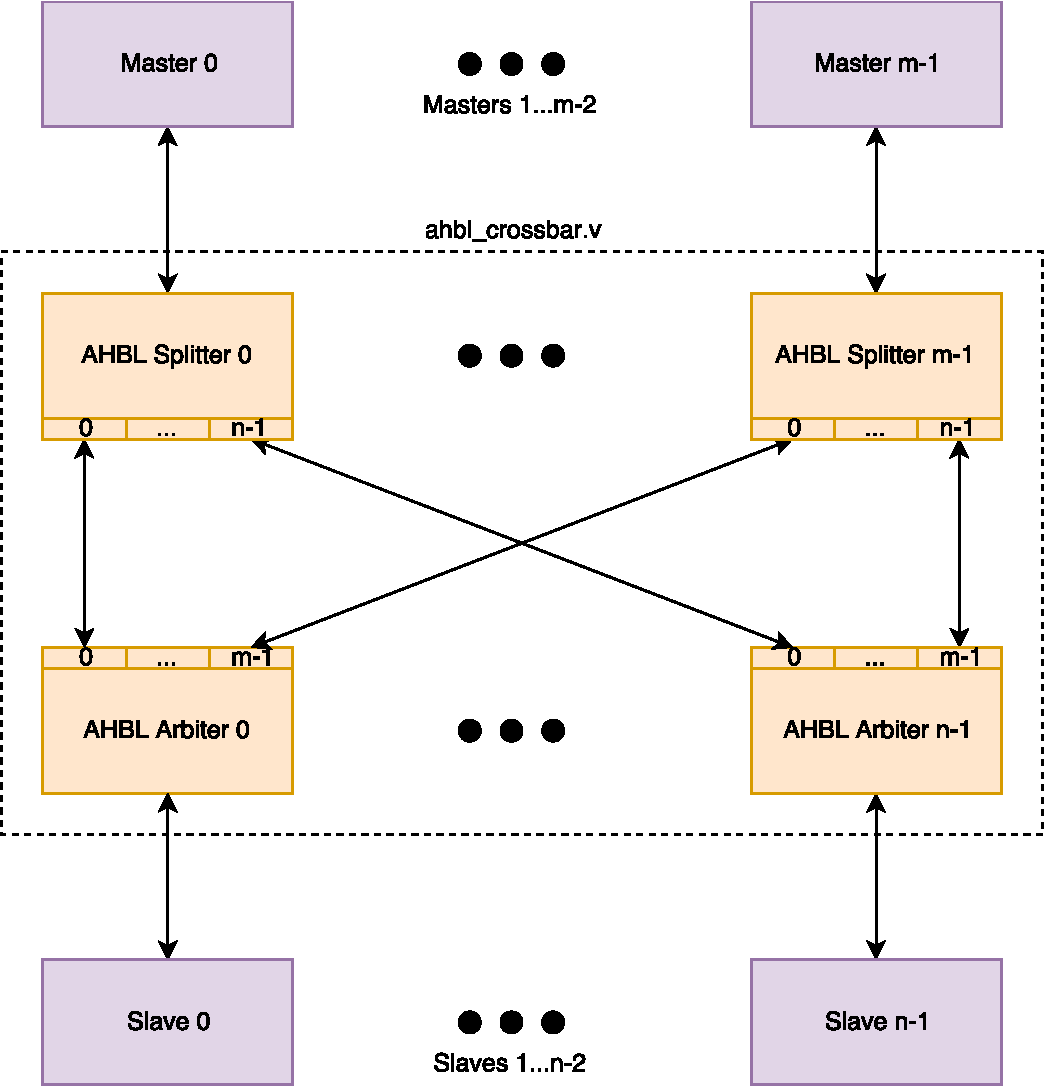
\includegraphics[width=0.6\textwidth]{diagrams/crossbar_structure.pdf}
\label{diagram:crossbar_structure}
\end{figure}

Each master is under the illusion that it is the only master in the system, but that slaves sometimes take longer to respond. During this waiting period, the slave may actually have fielded multiple transactions from higher-priority masters; this interaction is handled by the slave's AHB-Lite arbiter, and is transparent to the masters.

One of the crossbar's slave ports is attached to an AHBL-APB bridge. This bridge appears as a slave to the AHB portion of the bus fabric, and as a master to the APB portion. There are three main benefits to this scheme:

\begin{itemize}
	\item APB is fundamentally simpler
	\begin{itemize}
		\item This keeps peripheral gate count down
		\item The peripherals on the APB bus do not need the full AHB-Lite bandwidth anyway
	\end{itemize}
	\item Fewer AHB-Lite slaves
	\begin{itemize}
		\item There is a nonlinear area scaling associated with adding slaves to the AHB-Lite fabric
		\item This would also add extra gate delays to a fairly critical data path
	\end{itemize}
	\item One APB master
	\begin{itemize}
		\item AHB-Lite masters get arbitrated down to one inside the AHB-Lite crossbar. APB slaves do not care who is addressing them.
		\item Different masters accessing different APB slaves will have to queue to use the bridge, even though they could theoretically proceed simultaneously
		\item However, area/complexity vs performance tradeoff is more than worth it for slow peripherals
		\item Multi-master APB is easy to implement, but never used in practice, due to the above tradeoff
	\end{itemize}
\end{itemize}

The splitter and arbiter modules in the AHB-Lite crossbar can also be used on their own. Arbitrary multi-layer busfabric topologies should be possible with these two components.

Currently, the RISCBoy busfabric does not support AHB-Lite bursts (TODO), and the masters do not use them.

\subsection{AHB-Lite Primer}

For a full understanding of the bus standard used by RISCBoy, read through ARM's AMBA 3 AHB-Lite spec. This document is mirrored in the {\tt reference} folder in the GitHub repository, and gives a clear and comprehensive breakdown of AHB-Lite. However, the following overview should provide sufficient understanding of the standard to read through the Verilog.

Transactions take place in two phases, named the address phase and the data phase. During the address phase, the master asserts signals which control the nature of the transfer, such as the address, whether the transfer is a read or write, protection/permission information, the width of the data, and so on. During the data phase, data is asserted on either the read or write data bus ({\tt hrdata} and {\tt hwdata}), but never both. {\tt hrdata} is driven by the slave, and {\tt hwdata} by the master.

The central conceit of AHB-Lite is that these two phases are {\it pipelined}. Whilst the master is asserting or accepting data for an earlier transaction (currently in data phase), it concurrently asserts address and control information for a later transaction (currently in address phase). As is generally the case with pipelining, the goal is to enable higher clock frequencies with undiminished work-per-clock.

\begin{figure}[H]
\centering
\caption{AHB-Lite transfers, a simple example}
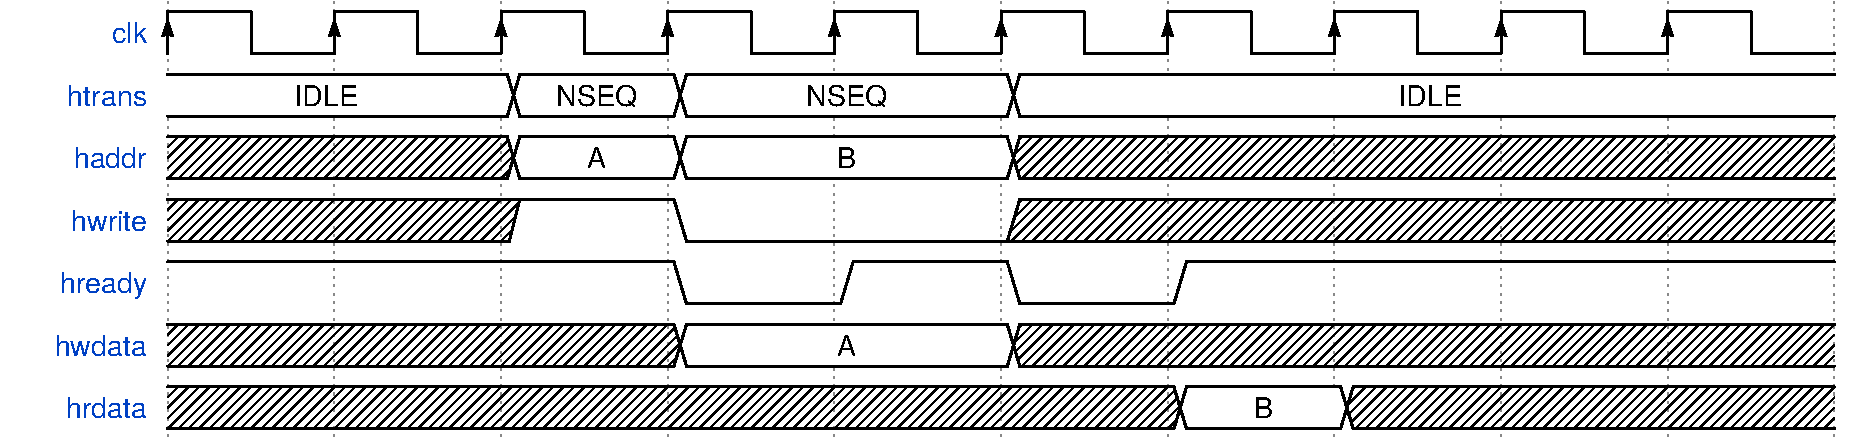
\includegraphics[width=0.9\textwidth]{waves/ahbl_basic.pdf}
\label{diagram:ahbl_basic}
\end{figure}

In figure \ref{diagram:ahbl_basic}, a master carries out two AHB-Lite transactions: a write to address A, followed by a read from address B. Only a subset of AHB-Lite signals are shown on the diagram. {\tt htrans}, {\tt haddr}, and {\tt hwrite} are driven by the master, during the address phase; the other two are data phase signals. {\tt htrans} indicates the type of transfer the master next wishes to perform, which is one of {\tt IDLE}, {\tt NSEQ} (non-sequential), {\tt SEQ} and {\tt BUSY}. The latter two are exclusive to burst transactions, which are not used in RISCBoy. (See the ARM spec if you do want details.)

Sometimes a slave is unable to service a request immediately, as shown in figure \ref{diagram:ahbl_basic_stall}. {\tt hready} is a data phase signal, which signifies the end of the current data phase.

\begin{figure}[H]
\centering
\caption{AHB-Lite transfers, simple example with stalling}
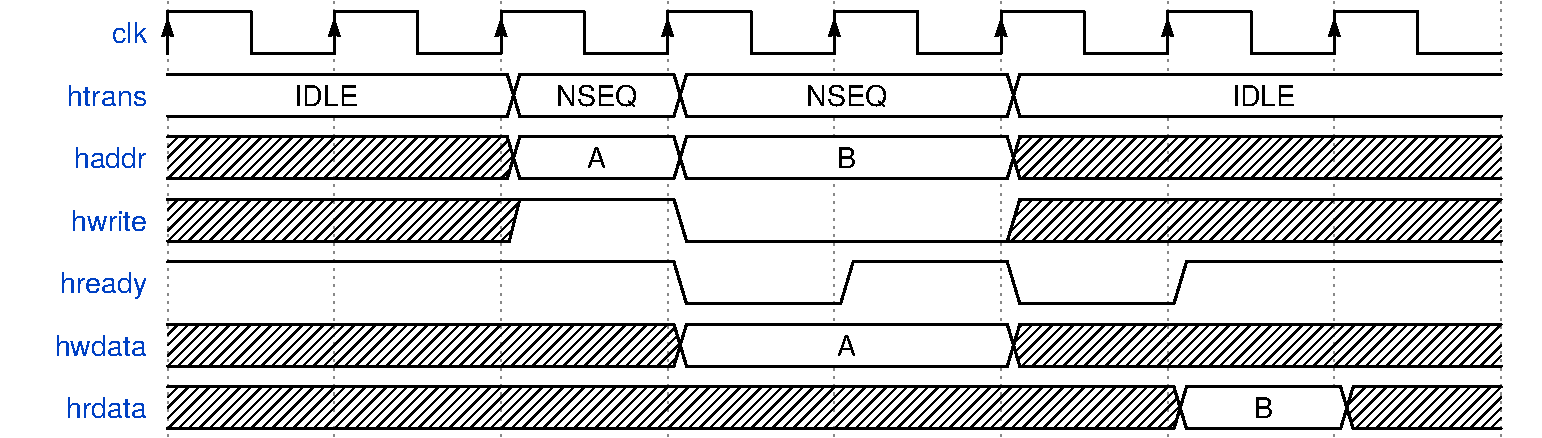
\includegraphics[width=0.9\textwidth]{waves/ahbl_basic_stall.pdf}
\label{diagram:ahbl_basic_stall}
\end{figure}

This slave needs two cycles to perform each data phase; perhaps it is an SRAM capable of running only at half the system clock speed. Therefore, {\tt hready} is low for one cycle, and high for the second (last) cycle of each data phase. The master drives {\tt hwdata} for the duration of A's data phase, waiting for the slave to signal completion. {\tt hrdata}, on the other hand, is invalid until the final cycle of a read data phase.

Note that an address phase does not complete until the preceding transfer's data phase completes. In figure \ref{diagram:ahbl_basic_stall}, address B (and associated address-phase signals) continue to be driven until the A data phase completes. {\tt IDLE} transactions do have a data phase, which always completes immediately. Consequently, {\tt hready} idles high while the bus is in an idle state. This is why A's address phase completes immediately in the figure.

In a practical system, there are multiple slaves. Each drives a signal called {\tt hreadyout}, to indicate that {\it that slave} is ready. The bus fabric tracks which slave the master is currently accessing in the data phase, and selects that slave's {\tt hreadyout} to be the global {\tt hready}. To see why this is necessary, think about the situation where a master is in data phase with one slave, and address phase with a different slave.

\subsection{Multi-Master Operation}

In a single-master busfabric, {\tt hready} is a global signal, which causes the entire AHB-Lite state machine (masters, slaves, fabric, the lot) to advance. Where multiple masters are concerned, {\tt hready} is more subtle; in part it is a per-master stall signal. At this point we need to be more specific about the relationship between {\tt hreadyout} and {\tt hready}.

Any AHB-Lite slave port (of which there is one on the master side of the splitter, $n$ on the master side of the arbiter, and one on each slave device) has an output called {\tt hreadyout}, which indicates the slave's readiness. Each of these ports also has an input called {\tt hready}, which indicates that the data phase is ending for the master who is connected to this slave (which does not mean that it is in data phase with {\it this} slave; it may be addressing this slave while in data phase with another). {\tt hready} is a function of {\tt hreadyout}s and bus state. The connections between masters, splitters, arbiters and slaves are shown in figure \ref{diagram:crossbar_structure}.

In the single-layer crossbar on RISCBoy, each system AHB-Lite slave is the slave of an arbiter, which is the slave of several splitters, each of which is the slave of a system master. As a general rule, the busfabric must filter system slaves' {\tt hreadyout}s up to each system master, tie {\tt hreadyout}s across to {\tt hready}s at the very top of the busfabric, and then distribute these {\tt hready} signals down to the correct system slaves.

\subsubsection{Multiple Masters, One Slave}

The arbiters are the most complex busfabric component, so it is instructive to consider interactions between multiple masters and a single slave, which are mediated by one arbiter. There are additional complexities when we combine arbiters and splitters to build a crossbar, which are discussed in the next section.

In figure \ref{diagram:ahbl_mm_simult1}, two masters attempt to access a single slave simultaneously. Assume that master 0 always wins address-phase arbitration:

\begin{figure}[H]
\centering
\caption{AHB-Lite transfers, two masters access one slave}
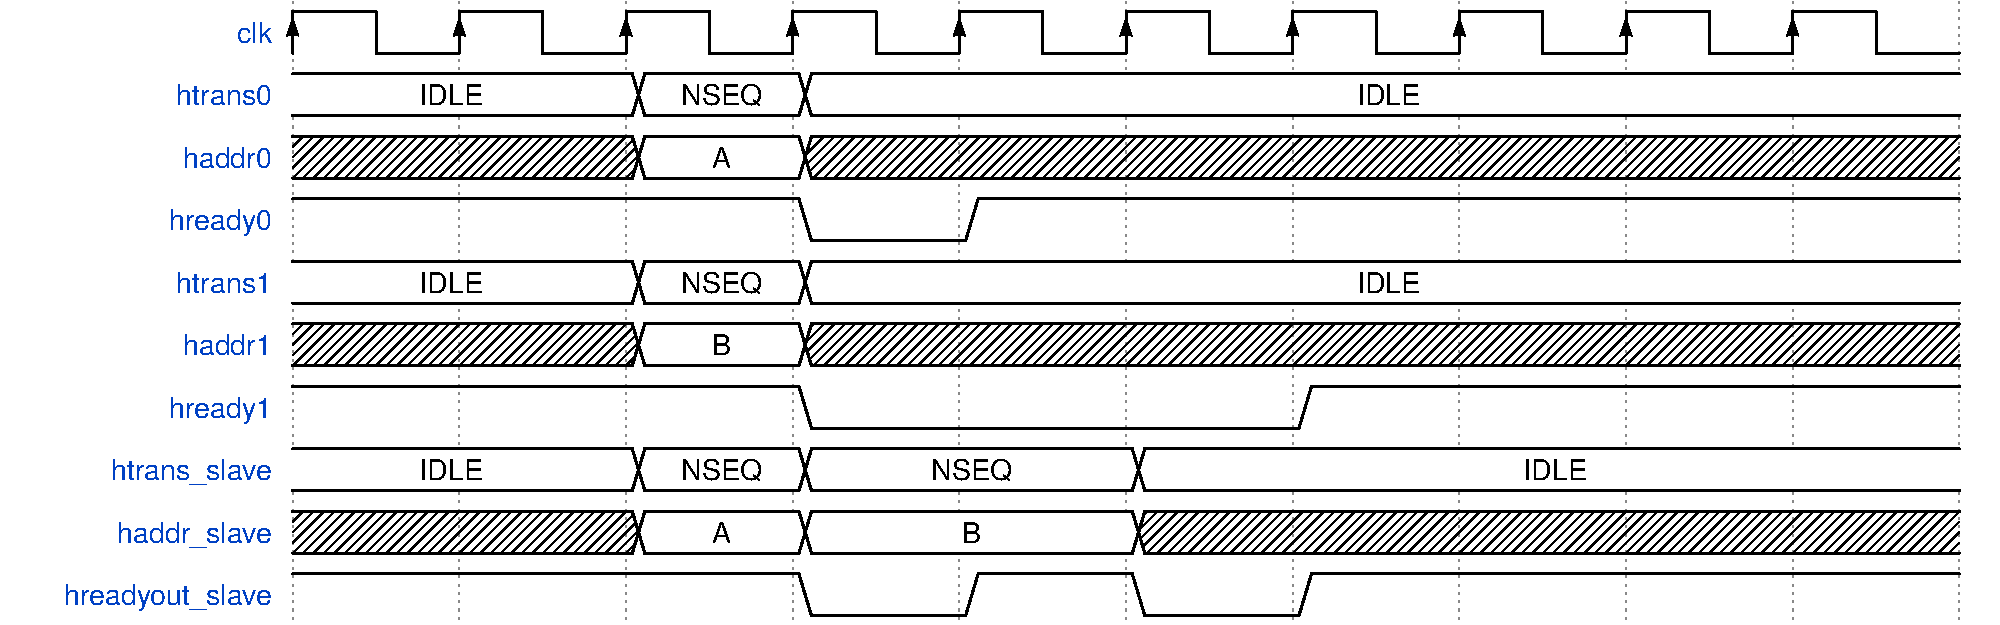
\includegraphics[width=0.9\textwidth]{waves/ahbl_mm_simult1.pdf}
\label{diagram:ahbl_mm_simult1}
\end{figure}

Again, we assume the slave requires 2 cycles to complete each data phase.

If we look at each master's trace, there is no indication at all that there is more than one master in the system: they present an address, and subsequently the transaction completes. Likewise, the slave neither knows nor cares that there are multiple masters: it simply carries out transactions according to the address-phase signals it sees. All of the smoke, mirrors and machinery are inside of the arbiter.

One odd feature of this trace is that, when the slave sees the address B, no master is asserting this address.

\begin{enumerate}
	\item Initially, both masters assert {\tt IDLE}; {\tt IDLE} data phases complete in one cycle
	\item {\tt IDLE} data phases are concurrent with A, B address phases, so these {\it also} complete immediately
	\item From the master 1's point of view, transaction B proceeds immediately to data phase.
	\item From both the master 0's and the slave's point of view, transaction A proceeds immediately to data phase
	\item Whilst the slave is in data phase for A, it is simultaneously in address phase for B
	\item When A data phase completes, master 0 is signaled, and B proceeds to data phase at the slave
	\item When B data phase completes, master 1 is signaled
\end{enumerate}

More concisely put, the first clock cycle of a given transaction's data phase may differ between the slave and master, but the {\it last} cycle of that data phase is always the same clock cycle. The slave address phase will occur some time between the master address phase starting, and the slave data phase starting. These are strong enough guarantees for correct operation.

Based on this discussion, the AHB-Lite arbiters need the facility to buffer one address-phase request, per master. A buffered request will be applied before any new requests from that master, but after any higher-priority requests. There is a nonzero hardware cost to this buffering, but there are clear engineering benefits to keeping this complexity confined to the arbiters, as they are the only component in the busfabric which is explicitly "multi master".

\begin{figure}[H]
\centering
\caption{AHB-Lite transfers, two masters access one slave, with low-priority back-to-back}
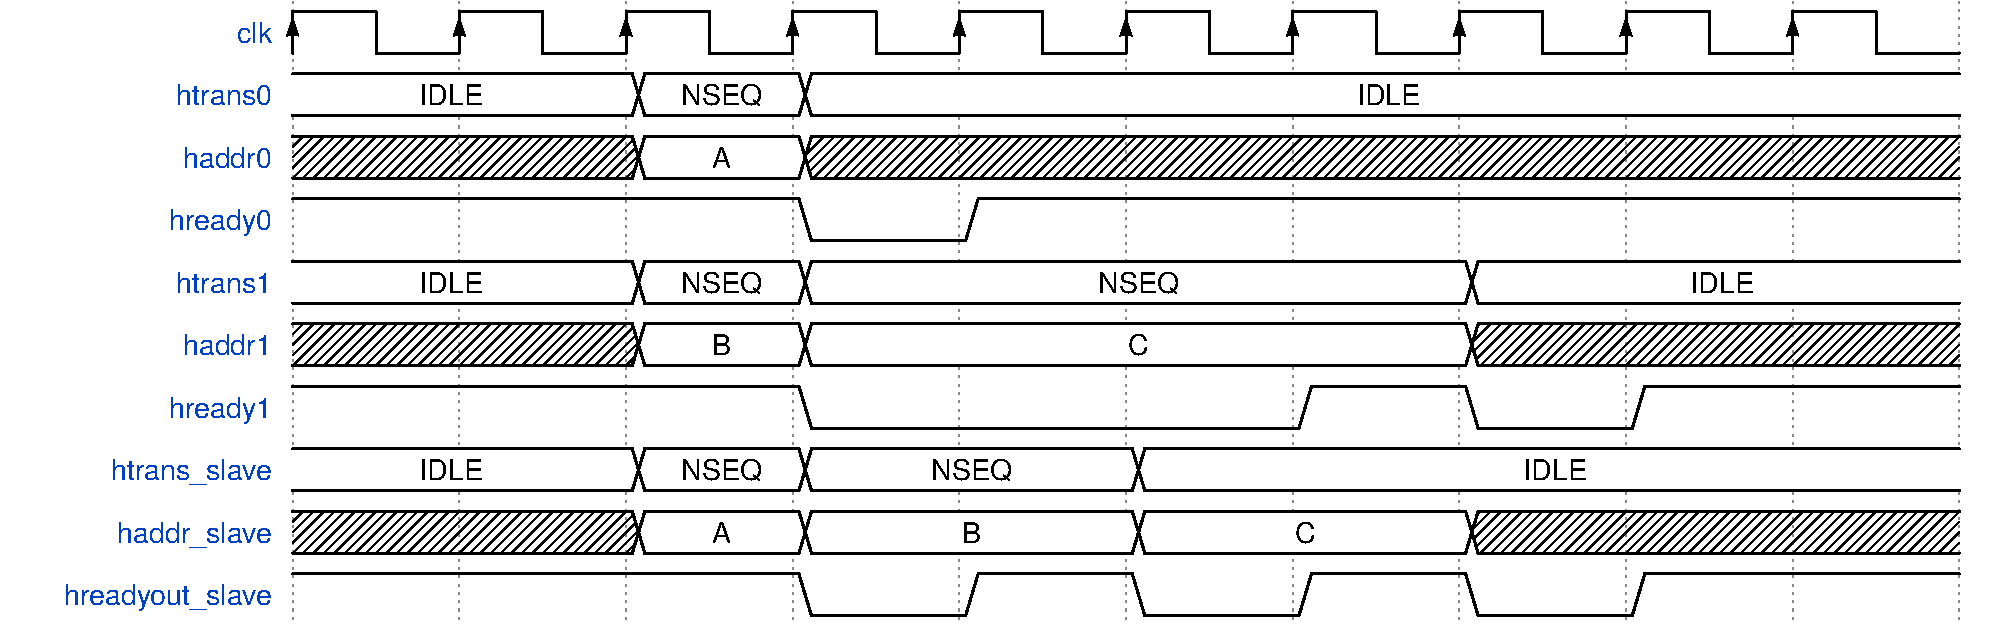
\includegraphics[width=0.9\textwidth]{waves/ahbl_mm_simult2.pdf}
\label{diagram:ahbl_mm_simult2}
\end{figure}

Figure \ref{diagram:ahbl_mm_simult2} shows the same sequence of events as figure \ref{diagram:ahbl_mm_simult1}, except master 1 now performs two back-to-back transactions. Once B's slave address phase completes, the arbiter's request buffer is cleared, and the C request passes transparently through the arbiter to the slave. Again, the only indication to master 1 of any master 0 activity is increased latency.

There is a different case which requires the arbiter's request buffer, shown in figure \ref{diagram:ahbl_mm_simult3}.

\begin{figure}[H]
\centering
\caption{AHB-Lite arbiter: simultaneous request buffer writes}
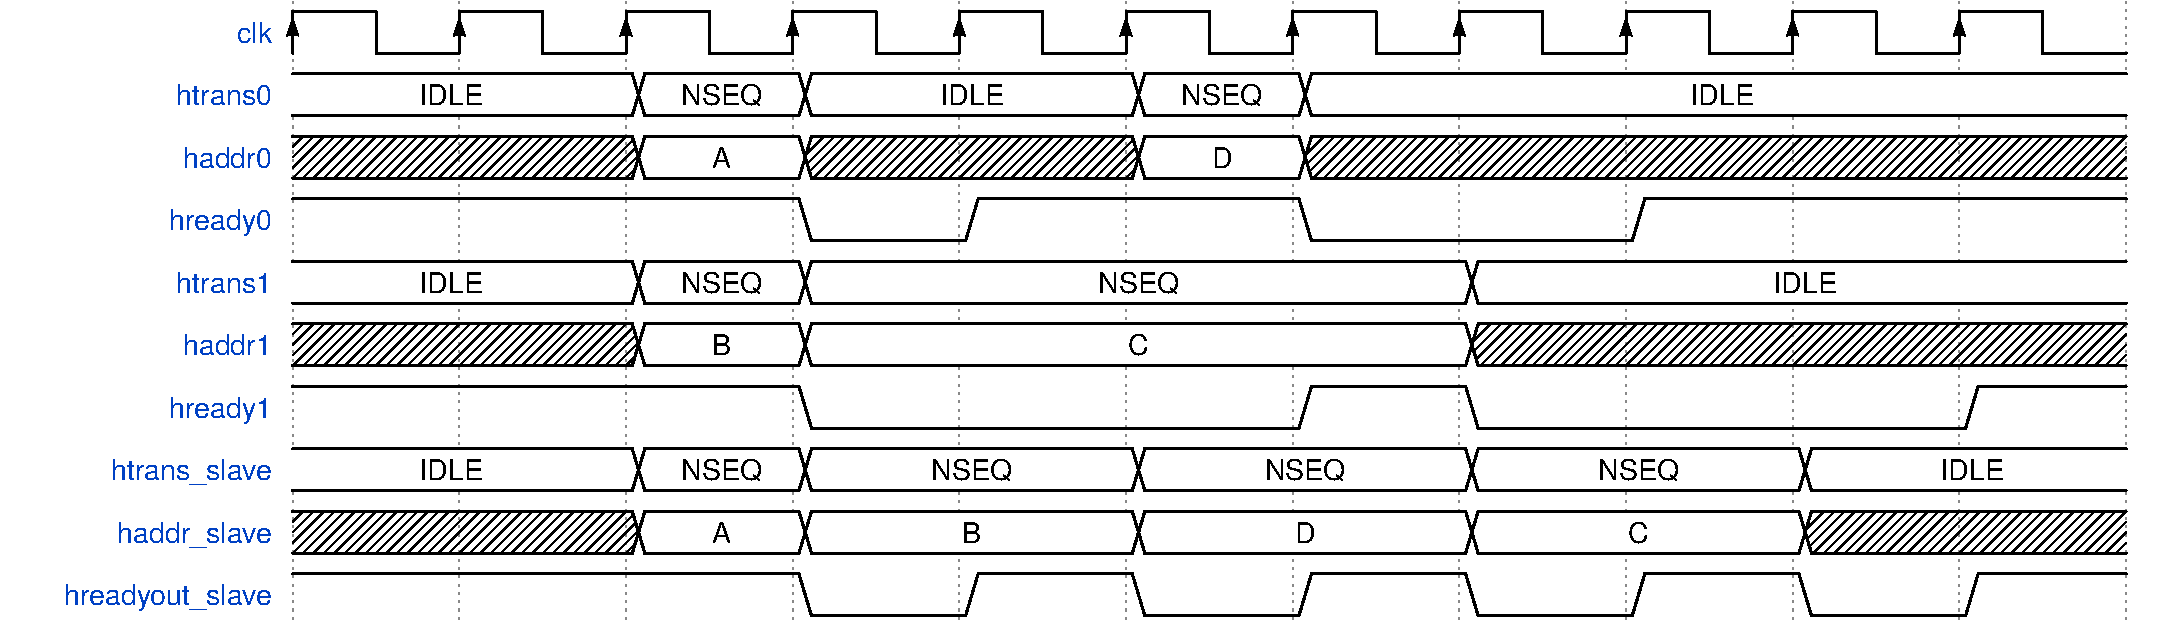
\includegraphics[width=0.9\textwidth]{waves/ahbl_mm_simult3.pdf}
\label{diagram:ahbl_mm_simult3}
\end{figure}

At the instant where D address phase is asserted, {\tt hready0} is high, because master 0 previously asserted an {\tt IDLE} transfer. However, the slave is not ready. In this case, the arbiter needs to buffer master 0's request, even though it is the highest-priority master. The buffered request is cleared once its slave address phase completes, as usual.

On the next cycle, B's data phase completes, and master 1 also considers this to be the end of the C address phase. The arbiter must write the C request into master 1's request buffer. Master 0's buffered request will continue to take priority over master 1's buffered request, until the first buffer is cleared.

There is one final case, for two masters accessing one slave, which is worth being aware of (figure \ref{diagram:ahbl_mm_latearrival}).

\begin{figure}[H]
\centering
\caption{AHB-Lite arbiter: late arrival of high priority request}
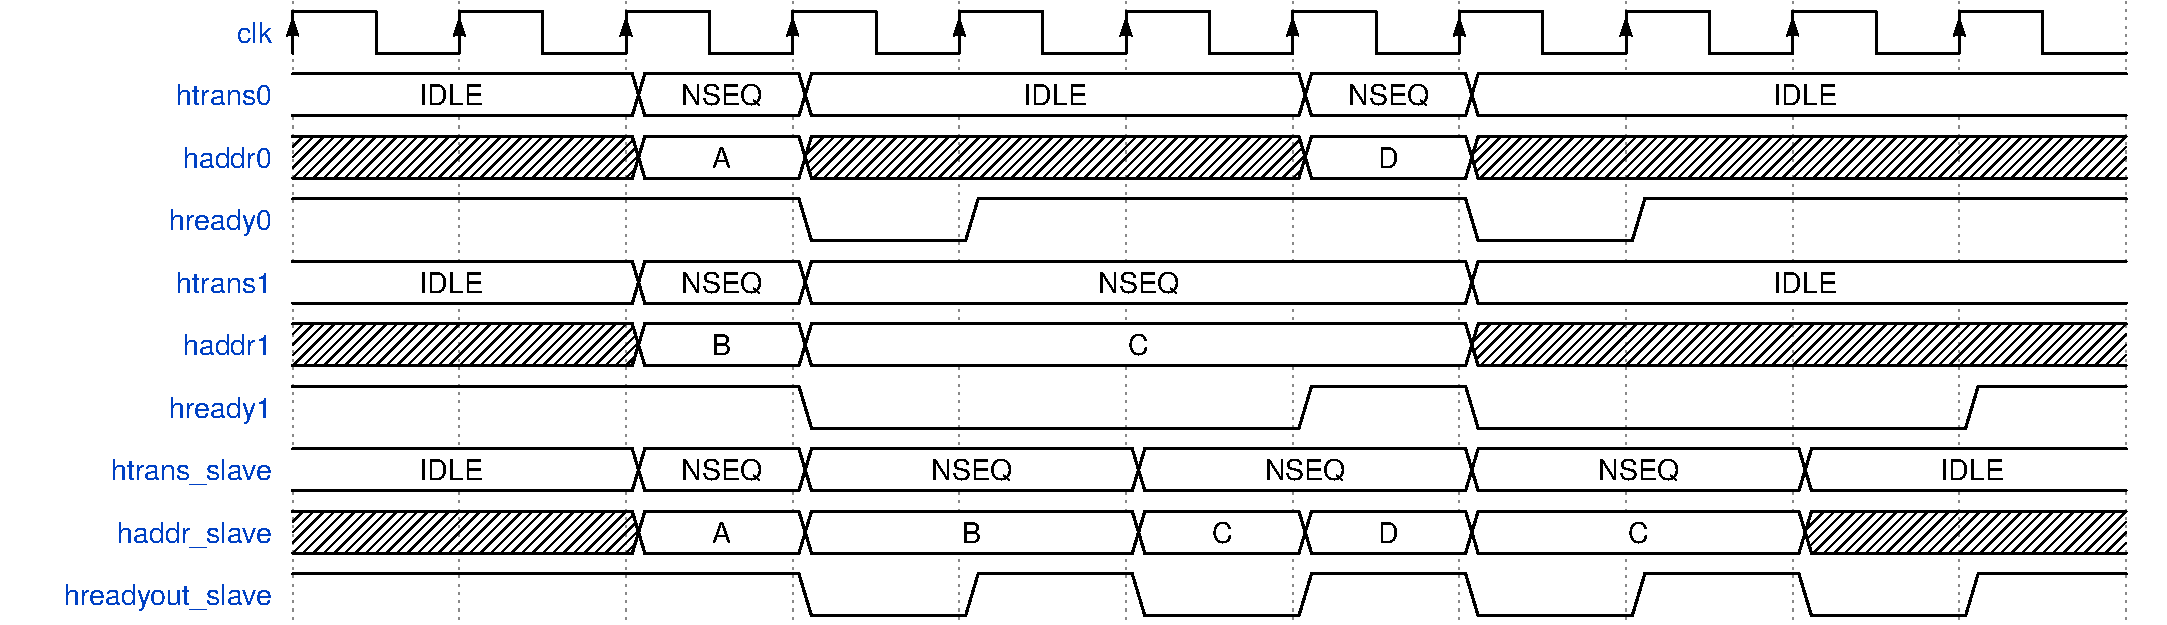
\includegraphics[width=0.9\textwidth]{waves/ahbl_mm_latearrival.pdf}
\label{diagram:ahbl_mm_latearrival}
\end{figure}

Whilst {\tt hreadyout} is low, the C address briefly appears on the slave bus, before being replaced by the higher-priority D request. \textbf{This is a departure from the AHB-Lite standard}, which stipulates the address must be constant during this time. This is deliberate, and easily amended. Slaves are generally insensitive to address-phase request during this time (as there is no performance benefit to latching APR before {\tt hreadyout}, due to the way the bus operates), and this avoids a priority inversion, reducing average latency for higher-priority masters. If you find something that this breaks, write me an angry email! I would be interested to see such a slave.

The D request causes the low-priority C request to be buffered; the B data phase completes on this cycle, hence, from master 0's point of view, the C address phase does too.

\subsubsection{Full Crossbar}

The previous section discussed some cases where multiple masters access a single slave, and showed how the arbiter safely navigates them. There are yet more issues to consider when multiple masters and multiple slaves are involved, which must be handled without added latency cycles, and with minimal extra gate delay.

For example, a master may be engaged in address phase with one arbiter and data phase with another arbiter simultaneously, via a splitter, and these two arbiters will not necessarily signal {\tt hreadyout} at the same time. Consequently, a master may have a positive {\tt hready}, filtered from its data phase arbiter, when its address phase arbiter has a negative {\tt hreadyout}, which requires action on the arbiter's part.

There is also the issue that being in data phase with an arbiter does not mean you are genuinely in data phase with the arbitrated slave; in fact, a very simple sequence of events (all masters {\tt IDLE} $\to$ all masters {\tt NSEQ}) will put all masters simultaneously in data phase with the same arbiter. The arbiter behaviour described in the previous section should allow us to abstract this away, provided we can deal with the first issue safely.

Splitters will filter their slaves' {\tt hreadyout}s based on which is currently in data phase, and present it on their own slave port. Arbiters will present their slave's {\tt hreadyout} on any master-facing ports which are in data phase with the arbiter, and will present ${\tt hreadyout} = 1$ on any idle ports.

Splitters will fan their {\tt hready} signal out to all of their slaves; a low {\tt hready} directed at a slave you are not engaged with is harmless.



\section{Pixel Processing Unit (PPU)}

{\it WARNING: This section rambles incoherently over a piece of hardware that does not yet exist, marking a complete departure from the preceding documentation}

\begin{figure}[!htb]
\centering
\caption{Pixel processing unit, block-level diagram}
\label{diagram:ppu_block}
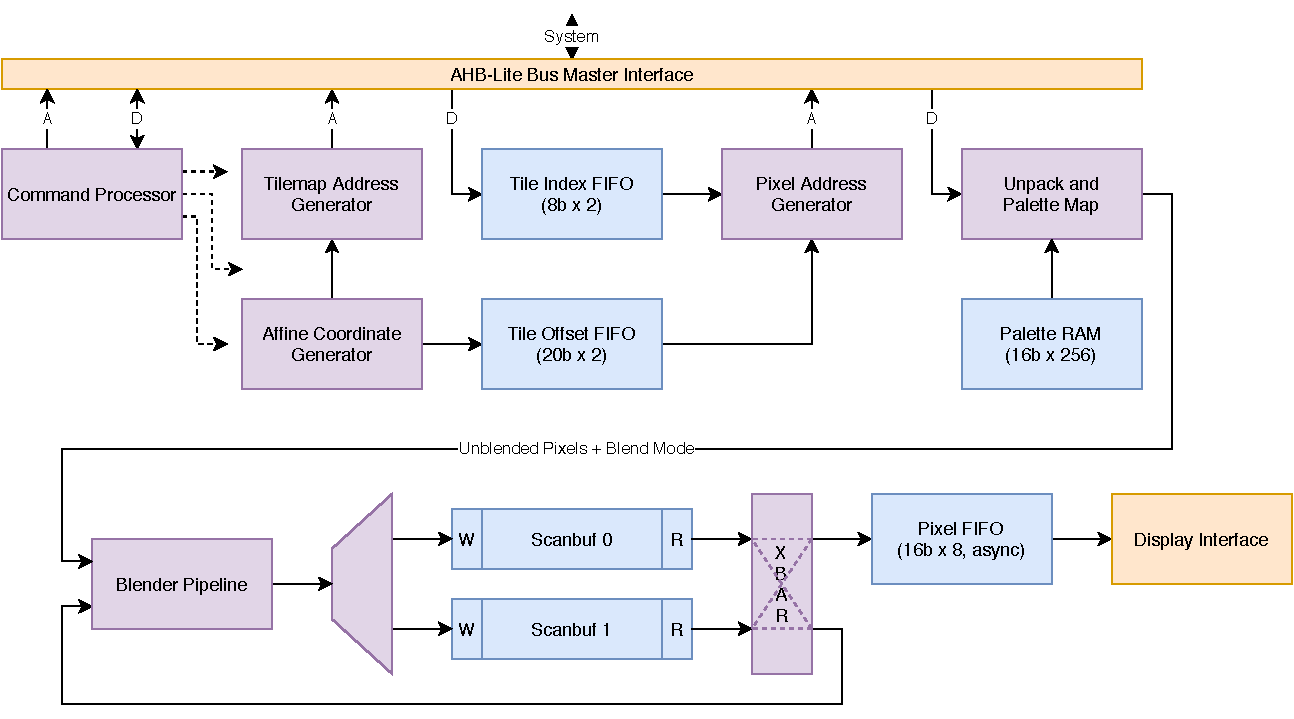
\includegraphics[width=\textwidth]{diagrams/ppu_block.pdf}
\end{figure}

Figure \ref{diagram:ppu_block} shows the high-level structure of the PPU. A number of independent sprite and background engines stream tile and pixel data from system memory, each producing a pixel stream which is continous in the case of the backgrounds, and generally sparse in the case of sprites. These multiple streams are blended according to transparency and layer order. Finally, any paletted pixels are looked up in the shared palette RAM, to produce full-colour pixels for the display.

The PPU makes no assumptions about display timing: for example, RISCBoy is currently equipped with a 320$\times$240 SPI LCD, which is driven continuously, with no horizontal or vertical blanking periods, as the SPI interface is the framerate bottleneck. The PPU continuously generates pixels at some rate which is hopefully higher than the display scan rate, and its timing is decoupled from the display via the pixel FIFO (as this is the narrowest point of the PPU, so the cheapest to buffer).

A key feature is the Poker: this is a simple raster-synchronised coprocessor that allows the PPU to modify its own configuration with pixel-perfect timing, enabling advanced rendering tricks such as in-scanline sprite multiplexing.

\subsection{Pixel Formats}

Internally, the PPU uses a single native pixel format, namely ARGB 1555 (see figure \ref{diagram:pixformat}), but to save bandwidth, the PPU can stream pixels from memory in a variety of formats, and convert internally. These range down to 1 bit per pixel, for both sprites and tiles. PPU memory accesses are \textbf{always little-endian}: for performance reasons the PPU performs the widest possible fetch, yielding multiple pixels each, which are numbered least-significant-first.

\begin{figure}[!htb]
\centering
\caption{PPU pixel formats}
\label{diagram:pixformat}
\begin{tabular}{r l}
	\raisebox{-1ex}[5ex][1.5ex]{
		\begin{bytefield}[endianness=big,bitformatting=\small, bitwidth=auto]{16}
		\bitheader{0,4,5,9,10,14,15} \\
		\bitbox{1}{A} \bitbox{5}{R} \bitbox{5}{G} \bitbox{5}{B}
		\end{bytefield}} & ARGB 1555, alpha = 0 when transparent \\
		\\
	\raisebox{-1ex}[5ex][1.5ex]{
		\begin{bytefield}[endianness=big,bitformatting=\small, bitwidth=auto]{16}
		\bitheader{0,4,5,9,10,14,15} \\
		\bitbox{1}{} \bitbox{5}{R} \bitbox{5}{G} \bitbox{5}{B}
		\end{bytefield}} & RGB 555, alpha bit is ignored (always opaque) \\
		\\
	\raisebox{-1ex}[5ex][1.5ex]{
		\begin{bytefield}[endianness=big,bitformatting=\small, bitwidth=auto]{8}
		\bitheader{0,1,2,4,5,6,7} \\
		\bitbox{1}{A} \bitbox{2}{R} \bitbox{3}{G} \bitbox{2}{B}
		\end{bytefield}} & ARGB 1232, alpha = 0 when transparent \\
		\\
	\raisebox{-1ex}[5ex][1.5ex]{
		\begin{bytefield}[endianness=big,bitformatting=\small, bitwidth=auto]{8}
		\bitheader{0,1,2,4,5,6,7} \\
		\bitbox{1}{} \bitbox{2}{R} \bitbox{3}{G} \bitbox{2}{B}
		\end{bytefield}} & RGB 232, alpha bit is ignored (always opaque) \\
		\\
	\raisebox{-1ex}[5ex][1.5ex]{
		\begin{bytefield}[endianness=big,bitformatting=\small, bitwidth=auto]{8}
		\bitheader{0,7} \\
		\bitbox{8}{Index}
		\end{bytefield}} & P8: an index into a table of 256 colours\\
		\\
	\raisebox{-1ex}[5ex][1.5ex]{
		\begin{bytefield}[endianness=big,bitformatting=\small, bitwidth=auto]{4}
		\bitheader{0,3} \\
		\bitbox{4}{Index}
		\end{bytefield}} & P4: an index into a table of 16 colours \\
		\\
	\raisebox{-1ex}[5ex][1.5ex]{
		\begin{bytefield}[endianness=big,bitformatting=\small, bitwidth=auto]{2}
		\bitheader{0,1} \\
		\bitbox{2}{Idx}
		\end{bytefield}} & P2: an index into a table of 4 colours \\
		\\
	\raisebox{-1ex}[5ex][1.5ex]{
		\begin{bytefield}[endianness=big,bitformatting=\small, bitwidth=auto]{1}
		\bitheader{0} \\
		\bitbox{1}{I}
		\end{bytefield}} & P1: an index into a table of 2 colours \\
		\\
\end{tabular}
\end{figure}

Background pixel format is configured per-background; sprite pixel format is configured globally.

For pixels smaller than one byte, the pixel order continues to be defined in a little-endian fashion, i.e. the least-significant pixel will be the first to be displayed. There is an additional constraint that all pixels be naturally aligned in memory. That is, pixel address modulo pixel size is zero.

A paletted pixel is transparent if:

\begin{itemize}
	\item The colour index is 0, and
	\item Transparency is enabled for that pixel source
\end{itemize}

So at e.g. 1 bit per pixel, it is possible to have either 2 colours, or 1 colour plus transparency. It is important that the transparency of a pixel is known as early as possible: this enables the PPU to perform layer composition before palette lookup, so only one palette lookup per {\it screen} pixel is required.


\subsection{Palettes}

The PPU contains a single hardware palette memory (PRAM). The PRAM is large enough to store 256 colours in RGB 555 format. Each pixel in a paletted image (see figure \ref{diagram:pixformat}) consists of an index into PRAM. The PPU looks these indices up before passing pixels to the screen; wide colour range is maintained at reduced bits per pixel.

Although there is only a single hardware palette, 256 colours in size, backgrounds and sprites can index this palette at an offset. PRAM may be initialised with e.g. multiple 16-colour tables at different (potentially overlapping) locations, giving effectively independent palettes.

PRAM can be addressed through the PPU's configuration interface, for configuration by the system. The PPU has priority access to the PRAM, so attempting to access PRAM during drawing may cause a lengthy stall. As with all PPU configuration state, it can also be updated by the Poker, using a {\tt poke} instruction; under ideal conditions the PPU can completely replace PRAM contents in 257 cycles.

\subsection{Layers}

Each background, and each sprite, can be individually assigned a layer number in the range $0 \leq n < N$, where $N$ is the layer count (configurable). The number of layers is wholly independent from the number of sprites, backgrounds, etc., and may be as little as 1. For each blended pixel, the blender observes non-transparent pixels from each source (sprite or background), and applies the following rules:

\begin{itemize}
	\item If there are no input pixels, output the display background colour.
	\item Else output the pixel with the lowest layer number
	\item If there are multiple pixels on the same layer:
	\begin{itemize}
		\item Sprites beat backgrounds
		\item Lower-numbered sprites beat higher-numbered
		\item Lower-numbered backgrounds beat higher-numbered
	\end{itemize}
\end{itemize}

Layer number can be thought of as depth into the screen. X is positive to the right, and Y is positive downward, so in a right-handed coordinate system, Z would be positive into the screen.

\subsection{Backgrounds}

Backgrounds are composed of tiles. Tiles are composed of pixels.

\begin{figure}[H]
\centering
\caption{PPU Background Coordinate System}
\label{diagram:ppu_bg_coords}
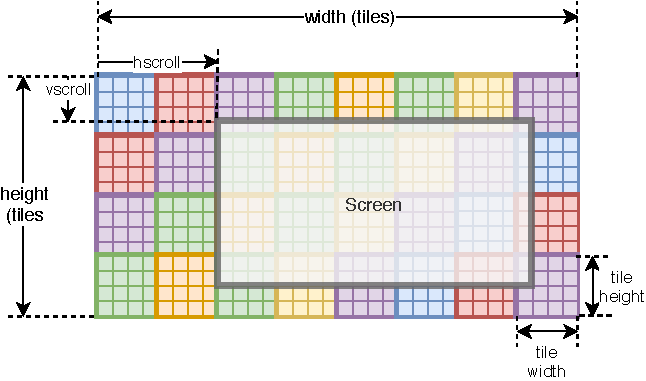
\includegraphics[width=0.7\textwidth]{diagrams/ppu_bg_coords.pdf}
\end{figure}

Each tile is a square image, the width and height of which (measured in pixels) is configured per-background, and is always a power of two. Tiles are stored in memory in a packed format: each tile is a sequence of pixels starting at the top left, proceeding left-to-right, then top-to-bottom. A region of memory packed with tile images (or sprites) will be referred to as an atlas. All images in a tile atlas are the same dimensions, and have the same pixel format.

The background itself is defined by:

\begin{itemize}
	\item A width and height, in tiles.
	\item A pointer to a tile atlas. The pointer is aligned to a one-tile boundary. The atlas contains up to 256 tiles.
	\item A pointer to a tilemap. The tilemap is $width \times height$ bytes in size, and byte-aligned.
\end{itemize}

For each pixel on the screen, the tilemap tells the PPU which tile should be at that location, and the tile image in the atlas tells the PPU the colour of each pixel in that screen tile.

The screen origin is offset into the background by configuring the horizontal and vertical scroll. This allows the game view to move smoothly over a fixed background. If the screen area overhangs the background, coordinates are wrapped. Unfortunately, the physical dimensions of the screen cannot be modified at run time.

\subsection{Sprites}

Sprites are small images which can be displayed at arbitrary screen coordinates; for example, the player character.

\subsection{Poker}
\label{section:ppu_poker}

The Poker is a programmable component of the PPU, inspired by the Amiga Copper. It allows the PPU to manipulate its own controls, with pixel-perfect timing. There are no restrictions on when this takes place, or what is changed.

This enables acrobatic feats such as multiplexing a single sprite back-to-back down a scanline. However, Poker execution does have a performance cost, as Poker instructions are fetched through the same memory interface as pixel data. Reconfiguring some pieces of hardware (e.g. a background engine) mid-scanline may trigger flushing of that hardware, which is also wasteful. Overuse may cause missed pixels.

Poker instructions reside in main system memory. Instructions are documented below. The instruction set is designed to be simple to decode and simple to generate dynamically, not to have high code density!

\subsubsection*{WAIT}

\begin{bytefield}[endianness=big,bitformatting=\tiny]{32}
\bitheader{0,11,12,23,24,31} \\
\bitbox{8}{{\tt WAIT}} \bitbox{12}{{\tt x}} \bitbox{12}{{\tt y}} \\
\end{bytefield}

Suspend execution, resuming immediately before pixel ({\tt x}, {\tt y}). For example {\tt WAIT 0, 0} will halt Poker execution until the start of the next frame. The Poker should generally spend most of its time in a suspended state, as it blocks pixel data fetches while it is executing.

Setting {\tt x} or {\tt y} to the all-ones bit pattern means "any". For example, the Poker may scan a block of sprite configuration at the start of every line, or change background colour at a certain point on every scanline.

Any pixels before ({\tt x}, {\tt y}) are unaffected by any changes the Poker may make. Once the Poker finishes poking, and goes back into the {\tt WAIT} state, all pixels after this point (inclusive of ({\tt x}, {\tt y}) take the new values into account.

\subsubsection*{POKE}

\begin{bytefield}[endianness=big,bitformatting=\tiny]{32}
\bitheader{0,15,24,31} \\
\bitbox{8}{{\tt POKE}} \bitbox{8}{{\tt count}} \bitbox{16}{{\tt addr}} \\
\bitheader{0, 31} \\
\bitbox{32}{{\tt data}} \\
\end{bytefield}

Write {\tt data} into the PPU's configuration address space, starting at {\tt addr}. The {\tt data} payload is ${\tt count}+ 1$ words in size. Absolutely any state can be modified, but beware that each pixel engine (sprite or background) will perform a reload when relevant config is written to.

For example, a background may have its tileset {\tt POKE}d at a certain point in each scanline, if there is a menu on the side of the screen which uses a font tilemap to draw text.

Some {\tt POKE}s are more expensive than others: it is possible to change the vertical scroll for every single pixel along a scanline, and this will produce the expected image. However, scrolling the screen invalidates the state of all sprites and backgrounds, which may cause slowdown if done too often.

Note that the Poker's program counter is mapped into the configuration address space; {\tt POKE} can be used to perform jumps.

\subsubsection*{SPRITE}

\begin{bytefield}[endianness=big,bitformatting=\tiny]{32}
\bitheader{0,7,8,15,16,23,24,31} \\
\bitbox{8}{{\tt SPRITE}} \bitbox{8}{count} \bitbox{8}{{\tt start}} \bitbox{8}{{\tt end}} \\
\bitheader{0, 31} \\
\bitbox{32}{{\tt addr}} \\
\end{bytefield}

Scan through {\tt count} sprite configuration words starting at {\tt addr} and assign them to sprites in range {\tt start}...{\tt end} if they intersect the current scanline. Disable remaining sprites. Stop scanning if {\tt end} is reached. If the display has a horizontal blanking period, this is the ideal time to perform {\tt SPRITE} scanning. This instruction is implemented with hardware already present in the PPU, so presents little extra cost.

This mechanism is similar to GameBoy OAM search. The effect is that the user can define a large number of virtual sprites -- more than are available in hardware -- and the PPU can draw all of these, as long as the number of sprites on one scanline is not greater than the hardware sprite count.

Alternatively, sprite allocation can be performed by software, and the sprites updated using a {\tt POKE} instruction. The {\tt POKE} approach is more flexible, and makes it easier to multiplex hard sprites within a single scanline.

\subsubsection*{SKIP}

\begin{bytefield}[endianness=big,bitformatting=\tiny]{32}
\bitheader{24,31} \\
\bitbox{8}{{\tt SKIP}} \bitbox{24}{TBD} \\
\end{bytefield}

Skip the following instruction, if the beam has reached some point. Full details TBD. It might be better to provide a conditional jump with a target, because not all of our instructions are the same length (especially {\tt POKE})

This allows Poker loops to be programmed, and makes the wait wildcard values much more useful.

\end{document}